\section{Metrics}
\label{sec:endpoint_metrics}
\begin{figure}[t]
 \centering
 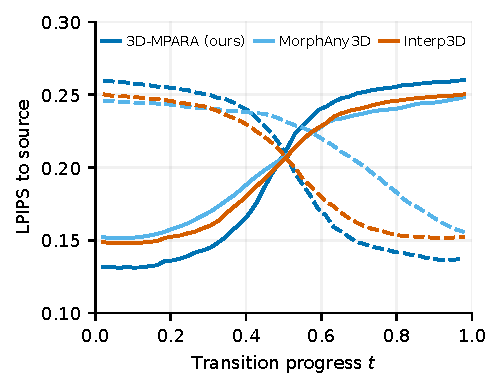
\includegraphics[width=\columnwidth]{figures/endpoint_distances_50.pdf}
 \caption{\textbf{Distances to both sources.} Color identifies the method;
 solid and dashed curves measure LPIPS to source 1 and source 2.
 Each curve averages 64 views over 50 pairs and displays the 48 generated
 intermediates. The canonical endpoint samples are omitted, with no
 connecting segments to $t=0$ or $t=1$.}
 \label{fig:distances50}
\end{figure}

We adopt the Interp Protocol from our teacher,
Interp3D~\cite{liu2026interp3d}, reporting FID~\cite{heusel2017fid} and
Interp3D's adaptation of perceptual path length (PPL)~\cite{karras2019stylegan}.
We also report perceptual distance variance (PDV) from
DiffMorpher~\cite{zhang2024diffmorpher}. FID compares concatenated renders
of two selected intermediates against those of both sources within each pair.
We also report mean LPIPS~\cite{zhang2018lpips} between consecutive
states along the complete path, including both canonical sources.

\begin{table*}[t]
\centering
\small
\setlength{\tabcolsep}{3pt}
\caption{Comparison on 50 held-out pairs. Values are means; \textbf{bold} and \underline{underline} mark the best and second mean in each column. FID, PPL, LPIPS, and PDV use the Interp Protocol; EPRE and TIME report both protocols. LPIPS, PPL, PDV, and EPRE include canonical endpoints. FID uses the concatenated-state definition. PDV is reported in units of $10^{-3}$. TIME is generation time per sequence in seconds. All metrics are minimized.}
\label{tab:standard}
\begin{tabular}{lrrrrrrrr}
\toprule
Method & FID $\downarrow$ & PPL $\downarrow$ & LPIPS $\downarrow$ & PDV ($10^{-3}$) $\downarrow$ & \multicolumn{2}{c}{EPRE $\downarrow$} & \multicolumn{2}{c}{TIME (s) $\downarrow$} \\
\cmidrule(lr){6-7}\cmidrule(lr){8-9}
& & & & & Interp Protocol & Dense Protocol & Interp Protocol & Dense Protocol \\
\midrule
MorphAny3D & \second{95.95} & \best{2.87} & \best{0.118} & $4.88$ & $0.33$ & $0.39$ & \second{182} & $1914$ \\
Interp3D & $96.02$ & \second{3.31} & \second{0.137} & \second{1.40} & \second{0.27} & \second{0.35} & $188$ & \second{897} \\
\methodname{} (ours) & \best{95.03} & $3.58$ & $0.148$ & \best{0.85} & \best{0.26} & \best{0.32} & \best{61} & \best{553} \\
\bottomrule
\end{tabular}
\end{table*}


\subsection{Endpoint Profile Error}
\label{sec:epre}

Image quality and local path regularity do not specify where an
intermediate lies close to its sources as the coefficient changes.
A sequence can change smoothly while staying close to one source or
departing from both. Our results illustrate this distinction: similar FID
and different PPL scores accompany distinct source-distance
profiles (Table~\ref{tab:standard}). The
qualitative sequences in Figure~\ref{fig:qualitative} and distance curves
in Figure~\ref{fig:distances50} motivate examining how each transition
leaves one source and approaches the other.

We introduce endpoint profile error (EPRE) to measure this progression.
Let $M(t)$ be the generated asset at progress $t\in[0,1]$, from $S_1$ to
$S_2$, and let $d(A,B)$ denote LPIPS averaged over matched camera views.
We normalize the distance to each source by their mutual distance:
\begin{equation}
 r_i(t)=\frac{d(M(t),S_i)}{d(S_1,S_2)},\qquad i\in\{1,2\}.
\end{equation}
A linear reference moves from distances $(0,1)$ to $(1,0)$, so its values
at progress $t$ are $(t,1-t)$. Writing $r_i=r_i(t)$, EPRE summarizes the
deviation from this reference across the transition:
\begin{equation}
 \epre=\sqrt{\tfrac12\!\int_0^1
       \big[(r_1-t)^2+(r_2-(1-t))^2\big]\,dt}.
 \label{eq:epre}
\end{equation}
Lower values mean closer agreement with the prescribed progression.
Normalization makes the score relative to the perceptual separation of
each source pair. We integrate over the sampled states using the
trapezoidal rule, including the canonical endpoints, and then average
pair scores.

EPRE complements the existing metrics: it describes source-relative
progression rather than image realism, geometric validity, or a unique
correct morph. The Dense Protocol samples the same reference more
densely, exposing behavior near the endpoints that the five central
intermediates of the Interp Protocol can miss.
